% file : noise_fem.tex
% author : Alicia Wang
% date : March 2014
%
% This file shows the code coupling idea with parallel domain decomposition applications
%
%----------------------------------------------------------------------------------

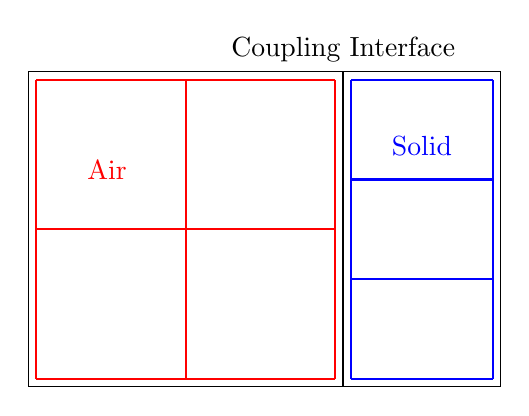
\begin{tikzpicture}

%\draw (0,0) -- (0,4) -- (4,4) -- (4,0) -- (0,0);
\draw (0,0) -- (6,0) -- (6,4) -- (0,4) -- (0,0);
\draw[thick] (4,0) -- (4,4) node[above, sloped] {Coupling Interface};

\node[red,  anchor=north] at (1, 3) {Air};
\node[blue, anchor=north] at (5, 3.3) {Solid};

\foreach \x in {0.1, 2, 3.9} 
  \foreach \y in {0.1, 2, 3.9} 
  { 
    \draw[red, thick]  (\x, 0.1) -- (\x, 3.9);
    \draw[red, thick]  (0.1, \y) -- (3.9, \y); 
  }
  
\foreach \y in {0.1, 1.367, 2.633, 3.9} 
{
  \draw[blue, thick] (4.1, \y) -- (5.9, \y);
}
 
\draw[blue, thick] (4.1, 0.1) -- (4.1, 3.9);
\draw[blue, thick] (5.9, 0.1) -- (5.9, 3.9);
	
\end{tikzpicture}
